\documentclass{exam}
\usepackage[utf8]{inputenc}
\usepackage[T1]{fontenc}
\usepackage{amsmath,amsfonts,amsthm} % Math packages for equations
\usepackage{tikz}
\usepackage{hyperref}
\usepackage{url}

\DeclareMathOperator{\diff}{d}
\DeclareMathOperator{\sign}{sgn}
\DeclareMathOperator*{\Res}{Res}
\DeclareMathOperator*{\reg}{reg}
\DeclareMathOperator*{\Ai}{Ai}
\DeclareMathOperator*{\Bi}{Bi}
\DeclareMathOperator*{\Disc}{Disc}
\newcommand{\calB}{\mathcal{B}}
\newcommand{\calL}{\mathcal{L}}

\usepackage{tikz}
\usetikzlibrary{decorations.markings}

\title{Lectures on Resurgence and Trans-Series}
\author{Marco Knipfer, University of Alabama}
\date{Week 15, Version: \today}

\begin{document}
\maketitle

\begin{questions}
    \setcounter{question}{10}
    \question (\textbf{Integral Definition of the Borel Transform\footnote{Following~\cite{Mas:2019dhl}}})

    For an asymptotic expansion
    \begin{equation}
        f(z) \sim \phi(z) = \sum_{n=0}^\infty \frac{a_n}{z^{n+1}}\, z\to+\infty\,,
        \label{eq:PhiAsymptExpansion}
    \end{equation}
    we had the \textit{Borel transform} defined as
    \begin{equation}
        \calB[\phi](\zeta) = \sum_{n=0}^\infty \frac{a_n}{n!} \zeta^n\,.
        \label{eq:BorelTransform}
    \end{equation}

    In this exercise we want to prove that
    \begin{equation}
        \calB[f](\zeta) = \frac{1}{2\pi i} \int_{\mathcal{C}_a} \diff\!z\, e^{z \zeta} f(z)\,,
        \label{eq:BorelIntegral}
    \end{equation}
    where $\mathcal{C}_a$ is a path $a+iy$, $y\in\mathbb{R}$ with a constant $a$ such that the path is to the right
    of all singularities of $f$.

    Check that the integral definition~(\ref{eq:BorelIntegral}) gives the same Borel transform as the usual
    definition~(\ref{eq:BorelTransform}).

    \textsc{Tipp}: Use the expansion~(\ref{eq:PhiAsymptExpansion}) and integrate using the residue theorem.

    \question{(Cauchy's Integral Formula and Branch Cuts)}\label{q:Cauchy}
    
    Say we have a function $f(z)$ that has a branch cut along the negative real axis with discontinuity $\Disc f(z)$
    and no other singularities (except the branch point at $z=0$).
    \begin{parts}
        \part{(Example: $\log$)}\\
        What is $\Disc f(z)$ for $f(z) = \log(z)$?

        \part{(Cauchy's Theorem)}\\
        \label{part:Cauchy}
        Show that the generic function $f(z)$ can be represented as
        \begin{equation}
            f(z) = - \frac{1}{2\pi i} \int_\delta^R \diff\!w\,\frac{\Disc f(-w)}{w + z} + I_\delta(z) + \mathcal{J}_R(z)\,.
        \end{equation}
        Use Cauchy's integral formula\footnote{See \textit{e.g.}~\cite{wiki:Cauchy}.}
        \begin{equation}
            f(a) = \frac{1}{2\pi i} \oint \frac{f(z)}{z-a}\diff z\,.
        \end{equation}
        and the contour given in figure~\ref{fig:contour}
                

        \begin{figure}
            \centering
            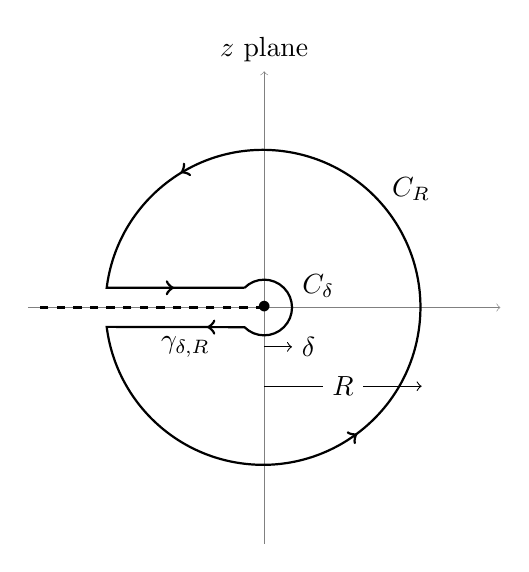
\begin{tikzpicture}[decoration={markings,
                    mark=at position 1cm with {\arrow[line width=1pt]{<}},
                    mark=at position 3.65cm with {\arrow[line width=1pt]{<}},
                    mark=at position 9.75cm with {\arrow[line width=1pt]{<}},
                    mark=at position 15.2cm with {\arrow[line width=1pt]{<}}
                }
                ]

                % The axes
                \draw[help lines,->] (-3,0) -- (3,0) coordinate (xaxis);
                \draw[help lines,->] (0,-3) -- (0,3) coordinate (yaxis);

                % The path
                \path[draw,line width=0.8pt,postaction=decorate] (-0.25,0.25) -- (-2,0.25) arc (172.875:-172.875:2) -- (-0.25,-0.25) arc (-135:135:0.353553) node[midway,above right]{$C_\delta$};

                \draw[->] (0,-1) -- (2,-1) node[midway,fill=white] {$R$};
                \draw[->] (0,-0.5) -- (0.353553,-0.5) node[right] {$\delta$};

                \draw[dashed,very thick] (0,0) node{$\bullet$} -- (-2.95,0);

                % The labels
                \node[above] at (yaxis) {$z$ plane};
                \node[below] at (-1,-0.25) {$\gamma_{\delta,R}$};
                \node[above,right] at (1.5,1.5) {$C_R$};
            \end{tikzpicture}
            \caption{Contour for part~\ref{q:Cauchy}~\ref{part:Cauchy}, figure from~\cite{Mas:2019dhl}.}
            \label{fig:contour}
        \end{figure}

    \end{parts}
    
\end{questions}

%\cite{Mas:2019dhl}
\begin{thebibliography}{666}
    \bibitem{Mas:2019dhl}
    R.~M.~Mas,
    ``Resurgence, a problem of missing exponential corrections in asymptotic expansions,''
    [arXiv:1904.07217 [hep-th]].
    \bibitem{wiki:Cauchy}
    Wikipedia contributors. Cauchy's integral formula. Wikipedia, The Free
    Encyclopedia. May 7, 2020, 09:44 UTC. Available at:
    \url{https://en.wikipedia.org/w/index.php?title=Cauchy\%27s_integral_formula&oldid=955351355.}
    Accessed July 30, 2020.
\end{thebibliography}

\end{document}
